\chapter{Loss Functions: The Interview Playbook}
\label{chap:loss_functions}

\begin{tldr}
Loss functions translate your learning objective into a mathematical optimization problem. The choice of loss function determines what your model learns to prioritize. This chapter covers classification losses (cross-entropy, focal, asymmetric), metric learning losses (contrastive, triplet, InfoNCE, ArcFace), ranking losses (BPR, LambdaRank), regression losses, and specialized losses for generation, segmentation, and knowledge distillation. Understanding \textit{when} to use each loss is as important as understanding the mathematics.
\end{tldr}

\section{The Philosophy of Loss Functions}
\label{sec:loss_philosophy}

\subsection{What Loss Functions Actually Do}

A loss function $\loss: \mathcal{Y} \times \mathcal{Y} \to \R_{\geq 0}$ measures the discrepancy between predictions $\hat{y}$ and targets $y$. The goal of training is to find parameters $\theta^*$ that minimize the expected loss:
\begin{equation}
\theta^* = \argmin_\theta \E_{(x,y) \sim \mathcal{D}}[\loss(f_\theta(x), y)]
\end{equation}

Four things to keep in mind at the whiteboard:

\begin{enumerate}
    \item \textbf{Proxy vs. True Objective}: The loss is almost always a \textit{proxy} for what we actually care about. We minimize cross-entropy but care about accuracy. We minimize MSE but care about perceptual quality.

    \item \textbf{Gradient Properties}: The loss must provide useful gradients. A loss that is flat everywhere or extremely sharp provides no useful learning signal.

    \item \textbf{Probabilistic Interpretation}: Many losses correspond to maximum likelihood estimation under specific distributional assumptions.

    \item \textbf{Implicit Regularization}: Different losses implicitly regularize differently. Cross-entropy with softmax encourages confidence; label smoothing penalizes it.
\end{enumerate}

\begin{keyinsight}
The loss function is how you communicate your objective to the optimizer. If you choose the wrong loss, you optimize for the wrong thing---even if training ``succeeds.'' A model trained with the wrong loss may achieve low training loss while failing at the actual task.
\end{keyinsight}

\subsection{A Taxonomy of Loss Functions}

\begin{figure}[H]
\centering
\begin{tikzpicture}[
    node distance=1.5cm,
    every node/.style={font=\small},
    box/.style={rectangle, draw, rounded corners, minimum width=2.5cm, minimum height=0.8cm, align=center},
    rootbox/.style={box, fill=lightblue, font=\bfseries},
    level1/.style={box, fill=lightgreen},
    level2/.style={box, fill=lightyellow, minimum width=2cm, font=\footnotesize}
]
    % Root
    \node[rootbox] (root) {Loss Functions};

    % Level 1
    \node[level1, below left=1.5cm and 3cm of root] (class) {Classification};
    \node[level1, below left=1.5cm and 0cm of root] (metric) {Metric Learning};
    \node[level1, below right=1.5cm and 0cm of root] (ranking) {Ranking};
    \node[level1, below right=1.5cm and 3cm of root] (other) {Specialized};

    % Level 2 - Classification
    \node[level2, below=0.8cm of class, xshift=-1.2cm] (ce) {Cross-Entropy};
    \node[level2, below=0.8cm of class, xshift=1.2cm] (focal) {Focal};
    \node[level2, below=1.8cm of class, xshift=-1.2cm] (bce) {BCE};
    \node[level2, below=1.8cm of class, xshift=1.2cm] (asym) {Asymmetric};

    % Level 2 - Metric
    \node[level2, below=0.8cm of metric, xshift=-1cm] (contr) {Contrastive};
    \node[level2, below=0.8cm of metric, xshift=1cm] (triplet) {Triplet};
    \node[level2, below=1.8cm of metric, xshift=-1cm] (infonce) {InfoNCE};
    \node[level2, below=1.8cm of metric, xshift=1cm] (arcface) {ArcFace};

    % Level 2 - Ranking
    \node[level2, below=0.8cm of ranking, xshift=-0.8cm] (bpr) {BPR};
    \node[level2, below=0.8cm of ranking, xshift=0.8cm] (lambda) {Lambda};
    \node[level2, below=1.8cm of ranking] (listwise) {Listwise};

    % Level 2 - Other
    \node[level2, below=0.8cm of other, xshift=-0.8cm] (mse) {MSE/MAE};
    \node[level2, below=0.8cm of other, xshift=0.8cm] (ctc) {CTC};
    \node[level2, below=1.8cm of other, xshift=-0.8cm] (dice) {Dice/IoU};
    \node[level2, below=1.8cm of other, xshift=0.8cm] (kd) {Distillation};

    % Edges
    \draw[-] (root) -- (class);
    \draw[-] (root) -- (metric);
    \draw[-] (root) -- (ranking);
    \draw[-] (root) -- (other);

    \draw[-] (class) -- (ce);
    \draw[-] (class) -- (focal);
    \draw[-] (class) -- (bce);
    \draw[-] (class) -- (asym);

    \draw[-] (metric) -- (contr);
    \draw[-] (metric) -- (triplet);
    \draw[-] (metric) -- (infonce);
    \draw[-] (metric) -- (arcface);

    \draw[-] (ranking) -- (bpr);
    \draw[-] (ranking) -- (lambda);
    \draw[-] (ranking) -- (listwise);

    \draw[-] (other) -- (mse);
    \draw[-] (other) -- (ctc);
    \draw[-] (other) -- (dice);
    \draw[-] (other) -- (kd);
\end{tikzpicture}
\caption{Taxonomy of loss functions covered in this chapter.}
\label{fig:loss_taxonomy}
\end{figure}

%==============================================================================
\section{Classification Losses}
\label{sec:classification_losses}
%==============================================================================

\subsection{Cross-Entropy Loss: The Foundation}

\textbf{What it is.} The default loss for multi-class classification. It measures how far your predicted probability distribution is from the true label. Cross-entropy equals minimizing KL divergence between true and predicted distributions.

\textbf{Key formula.} For $K$ classes, one-hot label $\vy$, and predictions $\hat{\vy} = \softmax(\vz)$:

\begin{mathresult}{Cross-Entropy Loss}
\begin{equation}
\loss_{\text{CE}}(\vy, \hat{\vy}) = -\sum_{k=1}^{K} y_k \log \hat{y}_k = -\log \hat{y}_c
\end{equation}
where $c$ is the index of the true class (i.e., $y_c = 1$).
\end{mathresult}

In terms of logits $\vz$ with true class $c$:
\begin{equation}
\loss_{\text{CE}}(\vz, c) = -z_c + \log\sum_{k=1}^{K} e^{z_k} = \log\sum_{k=1}^{K} e^{z_k} - z_c
\label{eq:ce_logits}
\end{equation}

\begin{keyinsight}
Minimizing cross-entropy is equivalent to minimizing KL divergence between the true distribution and the predicted distribution. Since entropy of a one-hot target is zero, the entire gap between the two distributions comes from the model's predictions.
\end{keyinsight}

\textbf{Gradient properties you should know:}
\begin{itemize}
    \item The gradient is simply $\hat{y}_k - y_k$: the difference between prediction and target.
    \item For the correct class, gradient magnitude is $|1 - \hat{y}_c|$---large when wrong, small when right. Self-correcting.
    \item Gradients for incorrect classes push their logits down proportionally to their predicted probability.
    \item All gradients are bounded in $[-1, 1]$, so CE never produces exploding gradients from the loss alone.
\end{itemize}

\subsubsection{Numerical Stability}

Direct computation of $\log(\softmax(\vz))$ is numerically unstable. The LogSumExp trick provides stability:
\begin{equation}
\log\sum_k e^{z_k} = m + \log\sum_k e^{z_k - m}, \quad m = \max_k z_k
\end{equation}

Now all exponents are $\leq 0$, preventing overflow. This is implemented as \texttt{log\_softmax} in modern frameworks.

\begin{warningbox}
Always use \texttt{CrossEntropyLoss} with raw logits or \texttt{log\_softmax} + \texttt{NLLLoss}. Never compute \texttt{softmax} followed by \texttt{log}---this loses numerical precision and can cause NaN gradients.
\end{warningbox}

\textbf{When to use.} Standard multi-class classification where exactly one class is correct.

\textbf{Pitfalls.} Sensitive to class imbalance (majority class dominates the gradient); encourages overconfidence on training data; the logit-based form is essential for numerical stability.

%------------------------------------------------------------------------------
\subsection{Binary Cross-Entropy (BCE)}
%------------------------------------------------------------------------------

\textbf{What it is.} Cross-entropy for binary or multi-label problems, applied independently per output.

\begin{mathresult}{Binary Cross-Entropy}
\begin{equation}
\loss_{\text{BCE}}(y, \hat{y}) = -y \log(\hat{y}) - (1-y) \log(1-\hat{y})
\end{equation}
where $y \in \{0, 1\}$ and $\hat{y} = \sigma(z) \in (0, 1)$.
\end{mathresult}

\textbf{Logits form.} Always use the logits form (\texttt{BCEWithLogitsLoss}) for numerical stability:
\begin{equation}
\loss_{\text{BCE-logits}}(y, z) = \max(z, 0) - yz + \log(1 + e^{-|z|})
\end{equation}

This fuses the sigmoid and log operations to avoid computing $\log(0)$.

\subsubsection{Multi-Label Classification}

For $K$ independent labels, apply BCE to each:
\begin{equation}
\loss_{\text{multi-label}} = \frac{1}{K}\sum_{k=1}^{K} \loss_{\text{BCE}}(y_k, \hat{y}_k)
\end{equation}

\begin{interviewq}
\textbf{Q: When do you use softmax cross-entropy vs. sigmoid BCE?}

\textbf{What the interviewer is testing:} Whether you understand the mutual exclusivity assumption baked into softmax, and can map problem structure to loss choice.

\textbf{A:} Use softmax CE when classes are \textbf{mutually exclusive} (exactly one correct answer, e.g., ``Is this a cat, dog, or bird?''). Use sigmoid BCE when labels are \textbf{independent} and multiple can be true (e.g., ``Does this image contain a cat? A dog? A bird?'').

The key distinction: softmax enforces $\sum_k \hat{y}_k = 1$, while sigmoid allows any combination. Using softmax for multi-label forces the model to ``choose'' between labels that aren't actually competing.

\textbf{Common follow-ups:} ``What if you have 10,000 classes---does softmax still work?'' ``How do you handle hierarchical labels?''
\end{interviewq}

\textbf{When to use.} Binary classification, multi-label classification, any setting where labels are independent.

\textbf{Pitfalls.} Must use logits form for stability; easy to accidentally apply softmax CE to a multi-label problem (a common bug).

%------------------------------------------------------------------------------
\subsection{Focal Loss}
%------------------------------------------------------------------------------

\textbf{What it is.} A modification of cross-entropy that down-weights easy examples so the model focuses on hard ones. Invented for object detection where 99.9\% of anchors are background.

\begin{mathresult}{Focal Loss}
\begin{equation}
\loss_{\text{FL}}(p_t) = -\alpha_t (1 - p_t)^\gamma \log(p_t)
\end{equation}
where $p_t = \hat{y}$ if $y=1$ else $1-\hat{y}$ (predicted probability for the true class), $\gamma \geq 0$ is the focusing parameter, and $\alpha_t$ is a class-balancing weight.
\end{mathresult}

\subsubsection{How the Modulating Factor Works}

The factor $(1-p_t)^\gamma$ does the heavy lifting:

\begin{itemize}
    \item \textbf{Easy examples} ($p_t \to 1$): Factor $\to 0$, loss heavily down-weighted
    \item \textbf{Hard examples} ($p_t \to 0$): Factor $\to 1$, full loss contribution
    \item \textbf{$\gamma = 0$}: Reduces to standard cross-entropy
\end{itemize}

\begin{table}[H]
\centering
\caption{Effect of focal loss modulating factor for different $\gamma$ values}
\begin{tabular}{c|cccc}
\toprule
$p_t$ & $\gamma=0$ & $\gamma=1$ & $\gamma=2$ & $\gamma=5$ \\
\midrule
0.9 & 1.0 & 0.1 & 0.01 & 0.00001 \\
0.5 & 1.0 & 0.5 & 0.25 & 0.03125 \\
0.1 & 1.0 & 0.9 & 0.81 & 0.59049 \\
\bottomrule
\end{tabular}
\end{table}

With $\gamma = 2$, an easy example with $p_t = 0.9$ contributes only 1\% of its original loss, while a hard example with $p_t = 0.1$ retains 81\%.

\subsubsection{When to Use Focal Loss}

\begin{itemize}
    \item \textbf{Extreme class imbalance}: Object detection (99.9\% background)
    \item \textbf{Dense prediction}: Semantic segmentation with rare classes
    \item \textbf{Multi-label with rare positives}: When positive rate per label is very low
\end{itemize}

\begin{warningbox}
Focal loss can under-optimize ``easy'' positive examples. If all positive examples matter equally (not just hard ones), standard cross-entropy with class weights may be preferable.
\end{warningbox}

\textbf{Pitfalls.} $\gamma$ is sensitive---too high and the model ignores everything except the hardest cases (which may include mislabeled data). Start with $\gamma = 2$, $\alpha = 0.25$.

%------------------------------------------------------------------------------
\subsection{Label Smoothing}
%------------------------------------------------------------------------------

\textbf{What it is.} Replace hard one-hot targets with soft targets that put a small amount of probability on every class. This prevents the model from becoming pathologically overconfident.

\textbf{Key formula:}
\begin{equation}
y_k^{\text{smooth}} = \begin{cases}
1 - \epsilon + \frac{\epsilon}{K} & \text{if } k = c \\
\frac{\epsilon}{K} & \text{otherwise}
\end{cases}
\end{equation}

\begin{example}
With $K=4$ classes, $\epsilon=0.1$:
\begin{itemize}
    \item Hard target: $[0, 0, 1, 0]$
    \item Smoothed target: $[0.025, 0.025, 0.925, 0.025]$
\end{itemize}
\end{example}

Label smoothing adds an entropy regularization term that prevents overconfidence.

\subsubsection{Effects of Label Smoothing}

\begin{enumerate}
    \item \textbf{Prevents overconfidence}: The model cannot achieve zero loss, limiting how extreme logits can become.

    \item \textbf{Better calibration}: Predictions become more calibrated (confidence matches accuracy).

    \item \textbf{Regularization}: Encourages more uniform (less confident) predictions, acting as regularization.

    \item \textbf{Softer decision boundaries}: Penalizes being ``too sure'' even when correct.
\end{enumerate}

\subsubsection{When to Use Label Smoothing}

\begin{itemize}
    \item Large models prone to overconfidence
    \item When calibrated probabilities matter (not just rankings)
    \item Knowledge distillation (makes teacher outputs more informative)
    \item \textbf{NOT for multi-label}: Not well-defined (targets already soft)
\end{itemize}

\textbf{Pitfalls.} Typical $\epsilon = 0.1$. Too large and you destroy the signal; too small and it has no effect. Not appropriate when you genuinely need the model to be highly confident.

%------------------------------------------------------------------------------
\subsection{Asymmetric Loss for Multi-Label}
%------------------------------------------------------------------------------

\textbf{What it is.} A focal-loss variant designed for multi-label classification, where each label independently has far more negatives than positives. It applies stronger down-weighting to easy negatives than to easy positives.

\begin{mathresult}{Asymmetric Loss}
\begin{equation}
\loss_{\text{ASL}} = \begin{cases}
(1-p)^{\gamma_+} \log(p) & \text{if } y = 1 \\
(p_m)^{\gamma_-} \log(1-p_m) & \text{if } y = 0
\end{cases}
\end{equation}
where $p = \sigma(z)$, $p_m = \max(p - m, 0)$ is probability shifted by margin $m$, $\gamma_+$ is focusing for positives, and $\gamma_- > \gamma_+$ is (stronger) focusing for negatives.
\end{mathresult}

\subsubsection{Components}

\begin{enumerate}
    \item \textbf{Asymmetric focusing}: $\gamma_- > \gamma_+$ down-weights easy negatives more than easy positives.

    \item \textbf{Probability shifting}: The margin $m$ (typically 0.05) means very easy negatives ($p < m$) are completely ignored.
\end{enumerate}

\subsubsection{Typical Hyperparameters}

\begin{itemize}
    \item $\gamma_+ = 0$ (no focusing on positives)
    \item $\gamma_- = 4$ (strong focusing on negatives)
    \item $m = 0.05$ (ignore negatives with $p < 0.05$)
\end{itemize}

\textbf{When to use.} Multi-label classification with long-tail label distributions (e.g., image tagging, document categorization).

\textbf{Pitfalls.} Three hyperparameters to tune ($\gamma_+$, $\gamma_-$, $m$). Start with the defaults above.

%------------------------------------------------------------------------------
\subsection{Class-Weighted Cross-Entropy}
%------------------------------------------------------------------------------

\textbf{What it is.} Weight the loss by inverse class frequency so rare classes get proportionally louder gradients.

\begin{equation}
\loss_{\text{weighted}} = -w_c \log\hat{y}_c
\end{equation}

\subsubsection{Common Weighting Schemes}

\begin{enumerate}
    \item \textbf{Inverse frequency}: $w_c = \frac{N}{N_c}$ where $N_c$ is count of class $c$

    \item \textbf{Inverse square root}: $w_c = \sqrt{\frac{N}{N_c}}$ (less aggressive)

    \item \textbf{Effective number}: $w_c = \frac{1-\beta}{1-\beta^{N_c}}$ for $\beta \in [0,1)$
\end{enumerate}

\begin{warningbox}
Extreme weights (e.g., 1000:1 for rare classes) can cause training instability. Consider combining with focal loss or using the effective number formulation with $\beta = 0.9999$.
\end{warningbox}

\textbf{When to use.} Moderate class imbalance where you want a simple, interpretable fix.

\textbf{Pitfalls.} Weights are dataset-level, not example-level---they don't distinguish hard from easy examples within a class (focal loss does).

%==============================================================================
\section{Metric Learning / Embedding Losses}
\label{sec:metric_losses}
%==============================================================================

Metric learning losses train embedding spaces where similar items are close and dissimilar items are far apart.

\subsection{Contrastive Loss}

\textbf{What it is.} The original pairwise metric learning loss. Takes pairs of items and pushes similar ones together, dissimilar ones apart (up to a margin).

\begin{mathresult}{Contrastive Loss}
For a pair $(x_i, x_j)$ with similarity label $y \in \{0, 1\}$ (1 = similar):
\begin{equation}
\loss_{\text{contrastive}} = y \cdot d(f(x_i), f(x_j))^2 + (1-y) \cdot \max(0, m - d(f(x_i), f(x_j)))^2
\end{equation}
where $d(\cdot, \cdot)$ is a distance metric (typically Euclidean) and $m$ is the margin.
\end{mathresult}

\subsubsection{Behavior Analysis}

\begin{itemize}
    \item \textbf{Similar pairs} ($y=1$): Loss = $d^2$. Minimize distance directly.
    \item \textbf{Dissimilar pairs} ($y=0$): Loss = $\max(0, m-d)^2$. Push apart until $d > m$.
\end{itemize}

\begin{figure}[H]
\centering
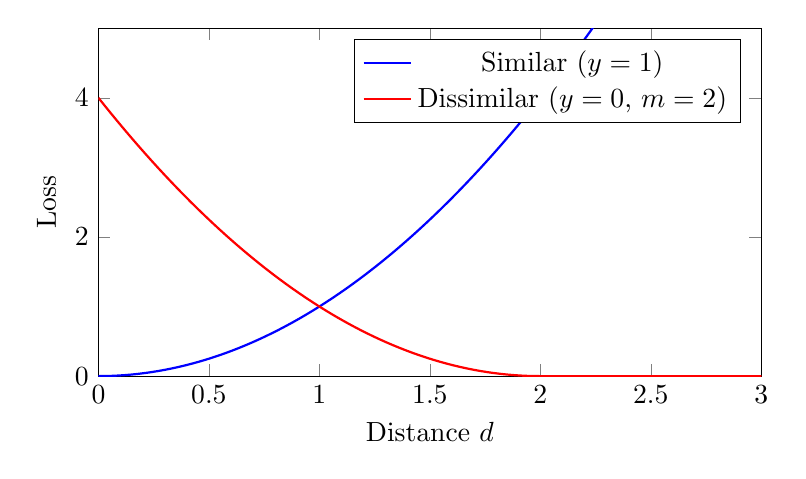
\begin{tikzpicture}
    \begin{axis}[
        xlabel={Distance $d$},
        ylabel={Loss},
        xmin=0, xmax=3,
        ymin=0, ymax=5,
        legend pos=north east,
        width=10cm,
        height=6cm
    ]
    % Similar pairs
    \addplot[domain=0:3, samples=100, thick, blue] {x^2};
    \addlegendentry{Similar ($y=1$)}

    % Dissimilar pairs (margin=2)
    \addplot[domain=0:3, samples=100, thick, red] {max(0, 2-x)^2};
    \addlegendentry{Dissimilar ($y=0$, $m=2$)}

    \end{axis}
\end{tikzpicture}
\caption{Contrastive loss as a function of distance for similar and dissimilar pairs.}
\end{figure}

\subsubsection{Limitations}

\begin{itemize}
    \item Requires careful pair sampling (balanced positives/negatives)
    \item Random pairs often trivially satisfied (uninformative)
    \item Only considers pairwise relationships
\end{itemize}

\textbf{When to use.} Verification tasks (same/different), small-scale metric learning.

\textbf{Pitfalls.} Largely superseded by triplet loss and InfoNCE for most applications. Margin $m$ is hard to tune.

%------------------------------------------------------------------------------
\subsection{Triplet Loss}
%------------------------------------------------------------------------------

\textbf{What it is.} Operates on triplets: anchor ($a$), positive ($p$), negative ($n$). Enforces that the anchor is closer to the positive than to the negative by at least a margin.

\begin{mathresult}{Triplet Loss}
\begin{equation}
\loss_{\text{triplet}} = \max(0, d(f(a), f(p)) - d(f(a), f(n)) + m)
\end{equation}
where $m > 0$ is the margin.
\end{mathresult}

\subsubsection{Geometric Interpretation}

The loss enforces: $d(a, n) > d(a, p) + m$

\begin{figure}[H]
\centering
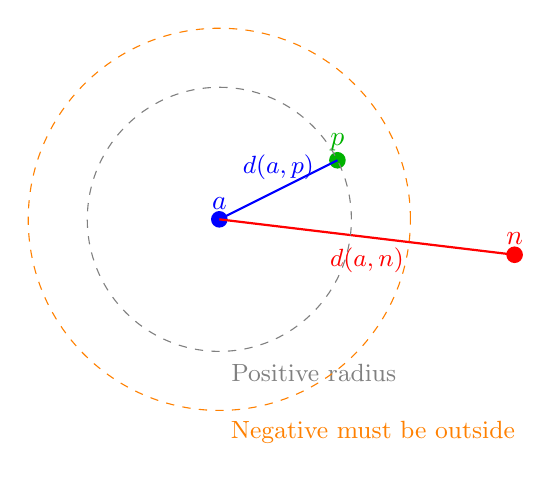
\begin{tikzpicture}[scale=1.5]
    % Points
    \fill[blue] (0,0) circle (2pt) node[above] {$a$};
    \fill[green!70!black] (1,0.5) circle (2pt) node[above] {$p$};
    \fill[red] (2.5, -0.3) circle (2pt) node[above] {$n$};

    % Distances
    \draw[blue, thick] (0,0) -- (1,0.5) node[midway, above, font=\small] {$d(a,p)$};
    \draw[red, thick] (0,0) -- (2.5,-0.3) node[midway, below, font=\small] {$d(a,n)$};

    % Margin visualization
    \draw[dashed, gray] (0,0) circle (1.118);
    \node[gray, font=\small] at (0.8, -1.3) {Positive radius};

    \draw[dashed, orange] (0,0) circle (1.618);
    \node[orange, font=\small] at (1.3, -1.8) {Negative must be outside};
\end{tikzpicture}
\caption{Triplet loss geometry: negative must be farther than positive by at least margin $m$.}
\end{figure}

\subsubsection{Triplet Mining Strategies}

The choice of triplets critically affects learning:

\textbf{Triplet Types.} Let $d_p = d(a, p)$ and $d_n = d(a, n)$.
\begin{itemize}
    \item \textbf{Easy}: $d_n > d_p + m$ (already satisfied, zero loss)
    \item \textbf{Hard}: $d_n < d_p$ (negative closer than positive!)
    \item \textbf{Semi-hard}: $d_p < d_n < d_p + m$ (violated but negative still farther)
\end{itemize}

\begin{table}[H]
\centering
\caption{Triplet mining strategies}
\begin{tabularx}{\textwidth}{lXX}
\toprule
\textbf{Strategy} & \textbf{Description} & \textbf{Trade-off} \\
\midrule
Random & Select random valid triplets & Many easy triplets, slow learning \\
Batch Hard & Hardest positive and negative per anchor in batch & Can cause collapse \\
Batch Semi-Hard & Hardest semi-hard negative per anchor & Best balance for most cases \\
Batch All & All valid triplets in batch & Computationally expensive \\
Offline Hard & Mine hard negatives periodically from full dataset & Expensive but effective \\
\bottomrule
\end{tabularx}
\end{table}

\begin{keyinsight}
\textbf{Semi-hard mining is usually best.} Easy triplets provide no gradient. Hard triplets can be too hard (e.g., mislabeled data) and cause training collapse. Semi-hard triplets are informative but not destabilizing.
\end{keyinsight}

\subsubsection{Margin Selection}

The margin $m$ controls the embedding space geometry:
\begin{itemize}
    \item \textbf{Small $m$}: Classes can be close, easier to satisfy
    \item \textbf{Large $m$}: Classes must be well-separated, may be hard to achieve
    \item \textbf{Typical}: $m \in [0.1, 1.0]$ for normalized embeddings
\end{itemize}

\textbf{When to use.} Retrieval, face verification, any setting where you have explicit positive/negative relationships and want fine-grained control over the embedding geometry.

\textbf{Pitfalls.} Training is fragile---mining strategy matters more than the loss formula itself. Requires large batches for effective in-batch mining.

%------------------------------------------------------------------------------
\subsection{InfoNCE / NT-Xent Loss}
%------------------------------------------------------------------------------

\textbf{What it is.} The workhorse of modern contrastive learning (SimCLR, CLIP, MoCo). Treats one positive pair against all other samples in the batch as negatives, forming a softmax-style classification over the batch.

\begin{mathresult}{InfoNCE / NT-Xent Loss}
For a positive pair $(x_i, x_j)$ among $N$ samples:
\begin{equation}
\loss_{\text{InfoNCE}} = -\log \frac{\exp(\text{sim}(z_i, z_j) / \tau)}{\sum_{k \neq i} \exp(\text{sim}(z_i, z_k) / \tau)}
\end{equation}
where $z = f(x)$ is the embedding, $\text{sim}$ is similarity (typically cosine), and $\tau$ is temperature.
\end{mathresult}

InfoNCE provides a lower bound on mutual information between views. Minimizing the loss maximizes a lower bound on mutual information, which tightens as the number of negatives increases.

\subsubsection{Temperature Analysis}

The temperature $\tau$ controls the ``hardness'' of the contrastive task:

\begin{figure}[H]
\centering
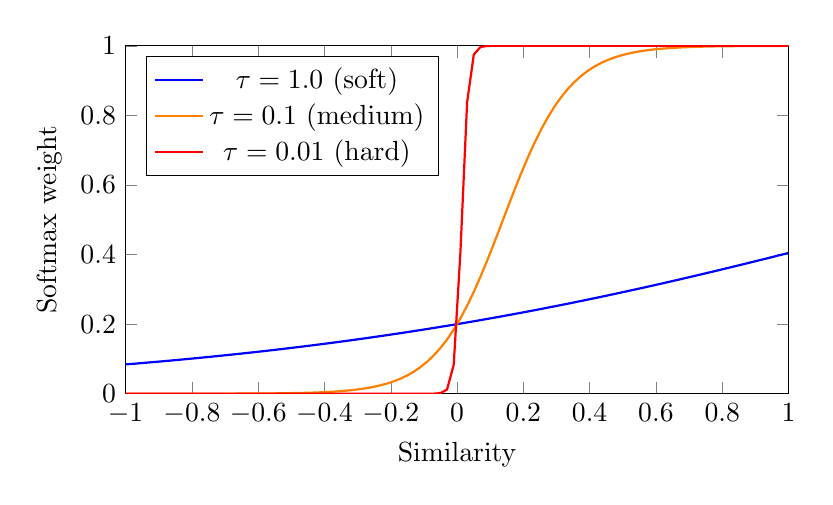
\begin{tikzpicture}
    \begin{axis}[
        xlabel={Similarity},
        ylabel={Softmax weight},
        xmin=-1, xmax=1,
        ymin=0, ymax=1,
        legend pos=north west,
        width=10cm,
        height=6cm
    ]
    % High temperature
    \addplot[domain=-1:1, samples=100, thick, blue] {exp(x/1) / (exp(x/1) + 4*exp(0/1))};
    \addlegendentry{$\tau=1.0$ (soft)}

    % Medium temperature
    \addplot[domain=-1:1, samples=100, thick, orange] {exp(x/0.1) / (exp(x/0.1) + 4*exp(0/0.1))};
    \addlegendentry{$\tau=0.1$ (medium)}

    % Low temperature
    \addplot[domain=-1:1, samples=100, thick, red] {exp(x/0.01) / (exp(x/0.01) + 4*exp(0/0.01))};
    \addlegendentry{$\tau=0.01$ (hard)}

    \end{axis}
\end{tikzpicture}
\caption{Effect of temperature on attention to similarities. Lower $\tau$ makes the loss focus on hard negatives.}
\end{figure}

\begin{itemize}
    \item \textbf{Low $\tau$ (0.01-0.1)}: Sharp distribution, dominated by hardest negatives
    \item \textbf{High $\tau$ (0.5-1.0)}: Soft distribution, all negatives contribute
    \item \textbf{Typical}: $\tau = 0.07$ (SimCLR), $\tau = 0.1$ (CLIP)
\end{itemize}

\subsubsection{In-Batch Negatives}

A key efficiency of InfoNCE: negatives come from other samples in the batch.

For batch size $B$:
\begin{itemize}
    \item Each sample has 1 positive (its augmented version)
    \item Each sample has $2(B-1)$ negatives (all other samples and their augmentations)
\end{itemize}

This makes training efficient but requires large batch sizes for sufficient negatives.

\begin{warningbox}
Large batch sizes in contrastive learning can cause GPU memory issues. Gradient accumulation does NOT help because you need all negatives in the same forward pass to compute the softmax denominator. Use gradient caching (decouple embedding computation from loss computation) instead.
\end{warningbox}

\begin{interviewq}
\textbf{Q: Why does SimCLR need large batch sizes?}

\textbf{What the interviewer is testing:} Whether you understand the connection between batch size and the quality of the contrastive objective, and whether you know alternatives.

\textbf{A:} SimCLR uses in-batch negatives for contrastive learning. With small batches, there are few negatives, making the contrastive task too easy. The model can achieve low loss by learning trivial features that happen to distinguish the few negatives in each batch. Large batches (4096+) provide diverse, challenging negatives that force learning of semantic features.

Alternative: MoCo uses a momentum-updated queue of negatives, decoupling negative count from batch size.

\textbf{Common follow-ups:} ``What's the memory cost of large batches?'' ``How does MoCo's momentum encoder avoid collapse?'' ``How does BYOL work without negatives at all?''
\end{interviewq}

\textbf{When to use.} Self-supervised pretraining (SimCLR, MoCo, CLIP), any contrastive learning setup where you have augmented views or paired data.

\textbf{Pitfalls.} Temperature $\tau$ is critical---too low and training becomes unstable; too high and the loss is too easy. Batch size directly affects quality of the bound.

%------------------------------------------------------------------------------
\subsection{ArcFace, CosFace, and SphereFace}
%------------------------------------------------------------------------------

\textbf{What it is.} Angular margin losses for highly discriminative embeddings. Standard softmax CE only requires the correct class logit to be the largest. Angular margin losses require it to be larger \textit{by a margin in angular space}, producing tighter, more separable clusters. They work by normalizing both weights and embeddings so the logit becomes $s \cdot \cos\theta$, where $\theta$ is the angle between the embedding and the class center, then adding a penalty margin.

\begin{mathresult}{Angular Margin Losses}
\begin{align}
\text{SphereFace (multiplicative):} \quad & \loss = -\log \frac{e^{s \cos(m\theta_c)}}{e^{s \cos(m\theta_c)} + \sum_{j \neq c} e^{s \cos\theta_j}} \\
\text{CosFace (additive cosine):} \quad & \loss = -\log \frac{e^{s(\cos\theta_c - m)}}{e^{s(\cos\theta_c - m)} + \sum_{j \neq c} e^{s \cos\theta_j}} \\
\text{ArcFace (additive angular):} \quad & \loss = -\log \frac{e^{s \cos(\theta_c + m)}}{e^{s \cos(\theta_c + m)} + \sum_{j \neq c} e^{s \cos\theta_j}}
\end{align}
\end{mathresult}

\subsubsection{Geometric Interpretation}

\begin{figure}[H]
\centering
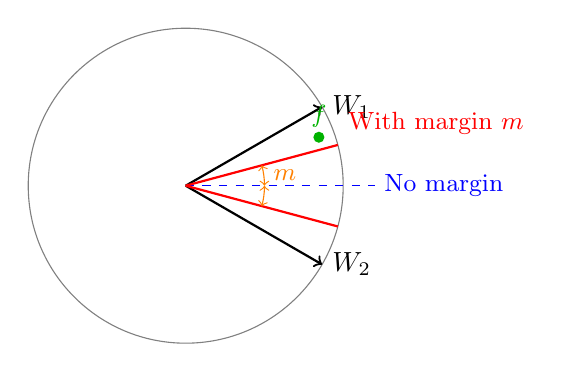
\begin{tikzpicture}[scale=2]
    % Unit circle
    \draw[gray, thin] (0,0) circle (1);

    % Class centers
    \draw[thick, ->] (0,0) -- (0.866, 0.5) node[right] {$W_1$};
    \draw[thick, ->] (0,0) -- (0.866, -0.5) node[right] {$W_2$};

    % Decision boundary without margin
    \draw[blue, dashed] (0,0) -- (1.2, 0) node[right, font=\small] {No margin};

    % Decision boundary with margin
    \draw[red, thick] (0,0) -- ({cos(15)}, {sin(15)}) node[above right, font=\small] {With margin $m$};
    \draw[red, thick] (0,0) -- ({cos(-15)}, {sin(-15)});

    % Margin angle
    \draw[<->, orange] (0.5, 0) arc (0:15:0.5) node[midway, right, font=\small] {$m$};
    \draw[<->, orange] (0.5, 0) arc (0:-15:0.5);

    % Sample embedding
    \fill[green!70!black] ({0.9*cos(20)}, {0.9*sin(20)}) circle (1pt) node[above, font=\small] {$f$};
\end{tikzpicture}
\caption{ArcFace adds an angular margin $m$, requiring the embedding to be closer to its class center by angle $m$ to achieve the same loss.}
\end{figure}

\subsubsection{Comparison}

\begin{table}[H]
\centering
\caption{Comparison of margin-based losses}
\begin{tabular}{lccc}
\toprule
\textbf{Loss} & \textbf{Margin Type} & \textbf{Typical $m$} & \textbf{Notes} \\
\midrule
SphereFace & Multiplicative angular & 4 & Hard to train \\
CosFace & Additive cosine & 0.35 & Easier to train \\
ArcFace & Additive angular & 0.5 & Best performance, most common \\
\bottomrule
\end{tabular}
\end{table}

\begin{keyinsight}
ArcFace is generally preferred because:
\begin{enumerate}
    \item The margin has constant effect across all angles (unlike CosFace where cosine is nonlinear)
    \item More stable training than SphereFace
    \item Clear geometric interpretation: ``embedding must be $m$ radians closer to correct class''
\end{enumerate}
\end{keyinsight}

\subsubsection{Scale Parameter}

The scale $s$ (typically 30-64) controls the concentration of the distribution:
\begin{itemize}
    \item Small $s$: Soft distribution, less discriminative
    \item Large $s$: Sharp distribution, more discriminative but may overfit
\end{itemize}

\textbf{When to use.} Face recognition, person re-identification, fine-grained visual retrieval---any problem with a fixed, large class set and where you need maximally discriminative embeddings.

\textbf{Pitfalls.} Requires a classification head during training (one weight vector per class), which doesn't scale to millions of classes without tricks (e.g., partial FC). Not suitable for open-set problems where classes change constantly.

\begin{interviewq}
\textbf{Q: You're building a visual search system for an e-commerce platform with 10M products. What loss function would you use for training the embedding model?}

\textbf{What the interviewer is testing:} Can you match loss functions to real-world system constraints? Do you think about scale, fine-grained similarity, and production requirements?

\textbf{A:} For large-scale visual search, I'd use \textbf{ArcFace} or \textbf{InfoNCE}, depending on the setup:

\begin{itemize}
    \item \textbf{ArcFace} if we have a fixed product catalog with class labels (each product = class). The angular margin produces highly discriminative embeddings for fine-grained visual similarity.
    \item \textbf{InfoNCE} if products are too numerous for a classification head, or if we want to learn from pairs/groups (e.g., same product from different angles). Scale with in-batch negatives + hard negative mining.
\end{itemize}

In practice, I'd likely use a two-stage approach: pre-train with InfoNCE on large data, then fine-tune with ArcFace on curated catalog data.

\textbf{Common follow-ups:} ``How do you handle new products added daily?'' ``What about multi-modal search (text + image)?''
\end{interviewq}

%==============================================================================
\section{Ranking Losses}
\label{sec:ranking_losses}
%==============================================================================

Ranking losses optimize the \textit{order} of items rather than absolute scores.

\subsection{Pairwise Ranking Loss}

\textbf{What it is.} A margin-based loss that ensures preferred items score higher than non-preferred items.

\begin{mathresult}{Margin Ranking Loss}
For preferred item $i$ over item $j$:
\begin{equation}
\loss = \max(0, -y(s_i - s_j) + m)
\end{equation}
where $y \in \{-1, +1\}$ indicates which item should rank higher, $s_i, s_j$ are scores, and $m$ is the margin.
\end{mathresult}

\textbf{When to use.} Simple ranking problems with explicit pairwise preferences.

\textbf{Pitfalls.} All pairs weighted equally---a swap at position 1 costs the same as a swap at position 1000.

\subsection{BPR Loss (Bayesian Personalized Ranking)}

\textbf{What it is.} Designed specifically for implicit feedback in recommender systems. Models the probability that a user prefers an interacted item over a non-interacted item.

\begin{mathresult}{BPR Loss}
For user $u$ with positive item $i$ and negative item $j$:
\begin{equation}
\loss_{\text{BPR}} = -\log \sigma(s_{ui} - s_{uj})
\end{equation}
where $\sigma$ is sigmoid and $s_{ui}$ is the predicted score for user-item pair.
\end{mathresult}

\textbf{When to use.} Recommender systems with implicit feedback (clicks, views, purchases). BPR only assumes clicked items are preferred over unclicked---it does not assume unclicked items are negative.

\textbf{Pitfalls.} Requires effective negative sampling. Uniform random negatives become too easy as training progresses; consider popularity-based or hard negative sampling.

\subsection{Listwise Losses}

\textbf{What they are.} Listwise approaches optimize entire rankings rather than individual pairs.

\subsubsection{ListNet}

Uses the top-one probability approximation from the Plackett-Luce model:
\begin{equation}
P(i \text{ ranked first} | s) = \frac{e^{s_i}}{\sum_j e^{s_j}}
\end{equation}

Loss is cross-entropy between predicted and true top-one probabilities.

\subsubsection{LambdaRank}

Key innovation: Weight pairwise gradients by the change in NDCG if items were swapped.

\begin{equation}
\lambda_{ij} = \frac{\partial \loss}{\partial s_i} = -\sigma(s_j - s_i) \cdot |\Delta\text{NDCG}_{ij}|
\end{equation}

\begin{keyinsight}
LambdaRank directly optimizes ranking metrics (NDCG) even though they're not differentiable. The $|\Delta\text{NDCG}_{ij}|$ weighting makes the model care more about swaps at the top of the ranking.
\end{keyinsight}

\textbf{When to use.} Search ranking, any setting where you care about NDCG or another position-sensitive metric.

\textbf{Pitfalls.} More complex to implement than pointwise/pairwise losses. The $\Delta\text{NDCG}$ computation adds overhead.

\begin{warningbox}
Ranking losses optimize \textit{order}, not \textit{scores}. If you need calibrated scores (e.g., click-through rate prediction for bidding), use pointwise cross-entropy with calibration, not a ranking loss.
\end{warningbox}

%==============================================================================
\section{Regression Losses}
\label{sec:regression_losses}
%==============================================================================

\subsection{Mean Squared Error (MSE / L2 Loss)}

\textbf{What it is.} The default regression loss. Penalizes errors quadratically, so large errors are penalized much more than small ones. Corresponds to assuming Gaussian noise.

\begin{mathresult}{MSE Loss}
\begin{equation}
\loss_{\text{MSE}} = \frac{1}{N}\sum_{i=1}^{N}(y_i - \hat{y}_i)^2
\end{equation}
\end{mathresult}

\textbf{Properties:}
\begin{itemize}
    \item \textbf{Outlier sensitive}: Squared errors penalize outliers heavily
    \item \textbf{Smooth everywhere}: Differentiable, stable gradients
    \item \textbf{Gradient}: $\frac{\partial \loss}{\partial \hat{y}} = -2(y - \hat{y})$ (linear in error)
    \item \textbf{Optimizes}: The conditional mean $\E[y | x]$
\end{itemize}

\subsection{Mean Absolute Error (MAE / L1 Loss)}

\textbf{What it is.} Linear penalty on errors. More robust to outliers than MSE. Corresponds to assuming Laplacian noise.

\begin{mathresult}{MAE Loss}
\begin{equation}
\loss_{\text{MAE}} = \frac{1}{N}\sum_{i=1}^{N}|y_i - \hat{y}_i|
\end{equation}
\end{mathresult}

\textbf{Properties:}
\begin{itemize}
    \item \textbf{Outlier robust}: Linear penalty, less sensitive than MSE
    \item \textbf{Non-smooth at zero}: Gradient undefined at $y = \hat{y}$
    \item \textbf{Gradient}: $\frac{\partial \loss}{\partial \hat{y}} = -\text{sign}(y - \hat{y})$ (constant magnitude)
    \item \textbf{Optimizes}: The conditional median
\end{itemize}

\begin{warningbox}
MSE optimizes the conditional mean, MAE optimizes the conditional median. If your target distribution is skewed (e.g., house prices, ad revenue), these give very different predictions. Choose based on what your business actually needs.
\end{warningbox}

\subsection{Huber Loss (Smooth L1)}

\textbf{What it is.} Best of both worlds: quadratic for small errors (smooth gradients, stable training), linear for large errors (outlier robust).

\begin{mathresult}{Huber Loss}
\begin{equation}
\loss_{\text{Huber}}(y, \hat{y}) = \begin{cases}
\frac{1}{2}(y - \hat{y})^2 & \text{if } |y - \hat{y}| \leq \delta \\
\delta|y - \hat{y}| - \frac{1}{2}\delta^2 & \text{otherwise}
\end{cases}
\end{equation}
\end{mathresult}

\begin{figure}[H]
\centering
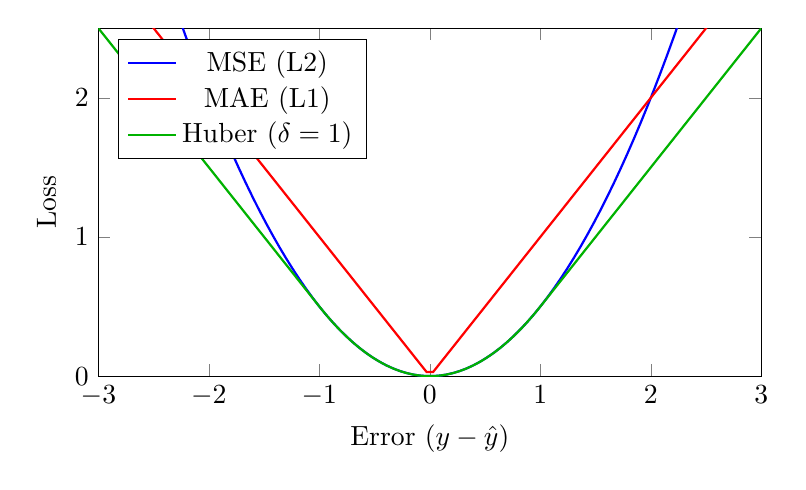
\begin{tikzpicture}
    \begin{axis}[
        xlabel={Error $(y - \hat{y})$},
        ylabel={Loss},
        xmin=-3, xmax=3,
        ymin=0, ymax=2.5,
        legend pos=north west,
        width=10cm,
        height=6cm
    ]
    % MSE
    \addplot[domain=-3:3, samples=100, thick, blue] {0.5*x^2};
    \addlegendentry{MSE (L2)}

    % MAE
    \addplot[domain=-3:3, samples=100, thick, red] {abs(x)};
    \addlegendentry{MAE (L1)}

    % Huber (delta=1)
    \addplot[domain=-3:-1, samples=50, thick, green!70!black] {abs(x) - 0.5};
    \addplot[domain=-1:1, samples=50, thick, green!70!black] {0.5*x^2};
    \addplot[domain=1:3, samples=50, thick, green!70!black] {abs(x) - 0.5};
    \addlegendentry{Huber ($\delta=1$)}

    \end{axis}
\end{tikzpicture}
\caption{Comparison of regression losses. Huber is quadratic near zero, linear for large errors.}
\end{figure}

\textbf{When to use.} Regression with noisy data or potential outliers. Also used in DQN (reinforcement learning) for stable value function training.

\textbf{Pitfalls.} The threshold $\delta$ is an extra hyperparameter. Default $\delta = 1$ is reasonable for standardized targets.

\subsection{Quantile Loss}

\textbf{What it is.} Asymmetric loss for predicting specific quantiles of the target distribution. Essential for uncertainty estimation and prediction intervals.

\begin{mathresult}{Quantile Loss}
\begin{equation}
\loss_\tau(y, \hat{y}) = \begin{cases}
\tau(y - \hat{y}) & \text{if } y \geq \hat{y} \\
(1-\tau)(\hat{y} - y) & \text{if } y < \hat{y}
\end{cases}
\end{equation}
where $\tau \in (0, 1)$ is the target quantile.
\end{mathresult}

\begin{itemize}
    \item $\tau = 0.5$: Median regression (equivalent to MAE)
    \item $\tau = 0.9$: 90th percentile (penalizes under-prediction more)
    \item $\tau = 0.1$: 10th percentile (penalizes over-prediction more)
\end{itemize}

Use multiple quantiles ($\tau = 0.1, 0.5, 0.9$) to get prediction intervals.

\textbf{When to use.} Forecasting with uncertainty bounds, risk-sensitive applications, any setting where you need prediction intervals.

\textbf{Pitfalls.} Quantile crossing---the 90th percentile prediction can end up below the 10th percentile. Use monotonic constraints or post-hoc sorting.

%==============================================================================
\section{Specialized Losses}
\label{sec:specialized_losses}
%==============================================================================

\subsection{CTC Loss (Connectionist Temporal Classification)}

\textbf{What it is.} For sequence-to-sequence tasks without explicit alignment (speech recognition, OCR). Marginalizes over all possible alignments between input and output.

\begin{mathresult}{CTC Loss}
\begin{equation}
\loss_{\text{CTC}} = -\log p(y | x) = -\log \sum_{\pi \in \mathcal{B}^{-1}(y)} p(\pi | x)
\end{equation}
where $\mathcal{B}$ is a mapping that removes blanks and repeated characters, and the sum is over all valid alignments.
\end{mathresult}

\subsubsection{Key Concepts}

\begin{enumerate}
    \item \textbf{Blank token}: Special token allowing ``no output'' at each timestep
    \item \textbf{Many-to-one mapping}: Multiple paths collapse to same output
    \item \textbf{Dynamic programming}: Efficient computation via forward-backward algorithm
\end{enumerate}

\begin{example}
Input: Audio of ``cat'' (100 frames)\\
Valid alignments:
\begin{itemize}
    \item c-c-c-a-a-t-t-t-$\epsilon$-$\epsilon$... $\to$ ``cat''
    \item $\epsilon$-c-$\epsilon$-a-$\epsilon$-t-$\epsilon$... $\to$ ``cat''
    \item c-a-a-a-t-$\epsilon$-$\epsilon$-$\epsilon$... $\to$ ``cat''
\end{itemize}
CTC sums probabilities over ALL valid alignments.
\end{example}

\textbf{When to use.} Speech recognition, OCR, any sequence labeling where input and output lengths differ and alignment is unknown.

\textbf{Pitfalls.} Assumes conditional independence between output tokens at each timestep (no language model built in). Often paired with an external language model at inference.

\subsection{Dice Loss / IoU Loss}

\textbf{What it is.} Region-overlap losses for segmentation. Unlike cross-entropy (which treats each pixel independently), Dice loss considers global overlap between prediction and ground truth.

\begin{mathresult}{Dice Loss}
\begin{equation}
\loss_{\text{Dice}} = 1 - \frac{2|A \cap B|}{|A| + |B|} = 1 - \frac{2\sum_i p_i g_i}{\sum_i p_i + \sum_i g_i}
\end{equation}
where $p$ is predicted probability and $g$ is ground truth.
\end{mathresult}

\subsubsection{Comparison with Cross-Entropy}

\begin{table}[H]
\centering
\caption{Cross-Entropy vs. Dice for segmentation}
\begin{tabularx}{\textwidth}{lXX}
\toprule
\textbf{Aspect} & \textbf{Cross-Entropy} & \textbf{Dice} \\
\midrule
Pixel independence & Treats each pixel independently & Considers global overlap \\
Class imbalance & Sensitive (background dominates) & Robust (ratio-based) \\
Gradients & Well-behaved everywhere & Can be noisy for small objects \\
Common practice & Combine: $\loss = \loss_{\text{CE}} + \lambda\loss_{\text{Dice}}$ & \\
\bottomrule
\end{tabularx}
\end{table}

\textbf{When to use.} Medical image segmentation, any segmentation task with significant class imbalance.

\textbf{Pitfalls.} Gradient is noisy when the predicted region is very small. Combine with CE for stable training.

\subsection{Knowledge Distillation Loss}

\textbf{What it is.} Transfer ``dark knowledge'' from a large teacher model to a small student model. The teacher's soft predictions reveal structure (e.g., ``dogs are more like cats than cars'') that hard labels miss.

\begin{mathresult}{Knowledge Distillation Loss}
\begin{equation}
\loss_{\text{KD}} = \alpha T^2 \cdot \KL(p_T^{(T)} \| p_S^{(T)}) + (1-\alpha) \cdot \loss_{\text{CE}}(y, p_S)
\end{equation}
where $p^{(T)} = \softmax(z/T)$ are temperature-scaled probabilities, $T$ is temperature, and $\alpha$ balances soft and hard targets.
\end{mathresult}

\subsubsection{Why Temperature Scaling?}

\begin{itemize}
    \item Teacher's hard predictions contain little information beyond the label
    \item Soft predictions reveal ``dark knowledge'': relative probabilities of wrong classes
    \item Higher $T$ produces softer distributions, revealing more structure
    \item $T^2$ scaling compensates for reduced gradient magnitude
\end{itemize}

\begin{example}
Teacher output (hard): ``dog'' = 0.99, ``cat'' = 0.008, ``car'' = 0.002\\
Teacher output ($T=4$): ``dog'' = 0.7, ``cat'' = 0.2, ``car'' = 0.1\\

The soft output tells the student: ``dogs and cats are similar, cars are different.''
\end{example}

\textbf{When to use.} Model compression, deploying large models to mobile/edge, training small models that punch above their weight.

\textbf{Pitfalls.} Temperature $T$ is critical: too low and soft targets look like hard labels (no benefit); too high and the distribution is uniform (no signal). Typical $T \in [3, 20]$. The $\alpha$ balance also matters---start with $\alpha = 0.5$.

%==============================================================================
\section{Loss Function Selection Guide}
\label{sec:loss_selection}
%==============================================================================

\begin{interviewq}
\textbf{Q: Your classification model gets 95\% accuracy but the loss curve shows the model is still decreasing slowly. Should you keep training?}

\textbf{What the interviewer is testing:} Understanding of the proxy-metric gap, overfitting risks, and calibration vs accuracy trade-offs.

\textbf{A:} Not necessarily. Several considerations:

\begin{enumerate}
    \item \textbf{Proxy vs. true objective}: Loss (cross-entropy) is a proxy for accuracy. Loss can keep decreasing while accuracy plateaus because the model is becoming more confident on already-correct predictions.
    \item \textbf{Overfitting risk}: Check validation loss. If training loss decreases but validation loss increases, you're overfitting.
    \item \textbf{Calibration}: Continued training often hurts calibration---the model becomes overconfident. If calibrated probabilities matter (e.g., medical, ranking), stop earlier.
    \item \textbf{Decision}: Use early stopping based on the \textit{actual metric you care about} on validation data, not training loss.
\end{enumerate}

\textbf{Common follow-ups:} ``How would you improve calibration?'' (Temperature scaling, label smoothing). ``What if you need both accuracy and calibration?''
\end{interviewq}

\begin{figure}[H]
\centering
\begin{tikzpicture}[
    node distance=0.8cm,
    every node/.style={font=\small},
    decision/.style={diamond, draw, aspect=2, inner sep=2pt, fill=lightyellow},
    result/.style={rectangle, draw, rounded corners, fill=lightgreen, minimum width=2cm},
    arrow/.style={->, thick}
]
    % Start
    \node[decision] (task) {Task type?};

    % Level 1
    \node[decision, below left=1.5cm and 2cm of task] (class) {Multi-class or multi-label?};
    \node[decision, below=1.5cm of task] (sim) {Pairwise or set-based?};
    \node[decision, below right=1.5cm and 2cm of task] (rank) {Pairwise or listwise?};

    % Classification branch
    \node[decision, below left=1cm and 0.5cm of class] (mc) {Imbalanced?};
    \node[decision, below right=1cm and 0.5cm of class] (ml) {Imbalanced?};

    % Results
    \node[result, below=0.8cm of mc, xshift=-1cm] (ce) {Cross-Entropy};
    \node[result, below=0.8cm of mc, xshift=1cm] (focal) {Focal Loss};
    \node[result, below=0.8cm of ml, xshift=-1cm] (bce) {BCE};
    \node[result, below=0.8cm of ml, xshift=1cm] (asym) {Asymmetric};

    % Similarity branch
    \node[result, below left=0.8cm and 0.3cm of sim] (triplet) {Triplet};
    \node[result, below right=0.8cm and 0.3cm of sim] (infonce) {InfoNCE};

    % Ranking branch
    \node[result, below left=0.8cm and 0.3cm of rank] (bpr) {BPR};
    \node[result, below right=0.8cm and 0.3cm of rank] (lambda) {LambdaRank};

    % Edges
    \draw[arrow] (task) -- node[above left] {Classification} (class);
    \draw[arrow] (task) -- node[left] {Similarity} (sim);
    \draw[arrow] (task) -- node[above right] {Ranking} (rank);

    \draw[arrow] (class) -- node[left] {Multi-class} (mc);
    \draw[arrow] (class) -- node[right] {Multi-label} (ml);

    \draw[arrow] (mc) -- node[left] {No} (ce);
    \draw[arrow] (mc) -- node[right] {Yes} (focal);
    \draw[arrow] (ml) -- node[left] {No} (bce);
    \draw[arrow] (ml) -- node[right] {Yes} (asym);

    \draw[arrow] (sim) -- node[left] {Pairwise} (triplet);
    \draw[arrow] (sim) -- node[right] {Batch} (infonce);

    \draw[arrow] (rank) -- node[left] {Pairwise} (bpr);
    \draw[arrow] (rank) -- node[right] {Listwise} (lambda);
\end{tikzpicture}
\caption{Decision tree for loss function selection.}
\end{figure}

\subsection{Quick Reference Table}

\begin{table}[H]
\centering
\caption{Loss function quick reference}
\begin{tabularx}{\textwidth}{lXl}
\toprule
\textbf{Scenario} & \textbf{Recommended Loss} & \textbf{Alternative} \\
\midrule
Multi-class, balanced & Cross-Entropy & Label Smoothing + CE \\
Multi-class, imbalanced & Focal Loss & Weighted CE \\
Multi-label, balanced & BCE & - \\
Multi-label, imbalanced & Asymmetric Loss & Focal + BCE \\
Face recognition & ArcFace & CosFace \\
General retrieval & InfoNCE & Triplet \\
Verification (same/different) & Contrastive & Triplet \\
Implicit feedback ranking & BPR & - \\
Search ranking & LambdaRank & ListNet \\
Regression, clean data & MSE & - \\
Regression, outliers & Huber & MAE \\
Regression, uncertainty & Quantile Loss & - \\
Segmentation & Dice + CE & IoU Loss \\
Sequence labeling & CTC & - \\
Model compression & KD Loss & - \\
\bottomrule
\end{tabularx}
\end{table}

\begin{interviewq}
\textbf{Q: You're building a product recommendation system with implicit feedback (clicks). What loss would you use and why?}

\textbf{What the interviewer is testing:} Whether you understand implicit vs. explicit feedback, the missing-data problem in recommendations, and multi-stage system design.

\textbf{A:} I would start with \textbf{BPR loss} for several reasons:
\begin{enumerate}
    \item \textbf{Designed for implicit feedback}: BPR optimizes pairwise preferences, which is exactly what clicks represent (clicked > not clicked).
    \item \textbf{Handles missing data correctly}: Unlike pointwise losses, BPR doesn't assume ``not clicked'' = negative; it only assumes clicked items are preferred over unclicked.
    \item \textbf{Scales well}: Negative sampling makes it efficient for large item catalogs.
\end{enumerate}

For the full system, I'd use a \textbf{two-stage approach}:
\begin{itemize}
    \item \textbf{Retrieval stage}: Two-tower model with InfoNCE/BPR for candidate generation
    \item \textbf{Ranking stage}: Listwise loss (or cross-entropy with calibration) for final ranking
\end{itemize}

\textbf{Common follow-ups:} ``How do you sample negatives?'' ``What if you also have explicit ratings?'' ``How do you handle position bias in clicks?''
\end{interviewq}
